\documentclass{beamer}
\usepackage{xeCJK}
\usepackage[colorlinks,linkcolor=blue,anchorcolor=red,citecolor=black]{hyperref}
\usepackage{color}
\usepackage{makecell}
\usepackage{multirow}
\usepackage{graphicx}
\usetheme{default}

\title{Optimize sequencing depth for shotgun metagenomics of pollination system by rarefaction, using a modular profiling pipeline}
% \subtitle{}
\author{Cong Liu}
% \institute{}
\date{2021.9}


\begin{document}

\begin{frame}
    \titlepage    
\end{frame}

\section{Introduction}

\begin{frame}{Bee health is a crucial issue}
    \begin{figure}
        \includegraphics[width=0.9\textwidth]{../Figures/BeeEconomicDecline.png}
    \end{figure}
    \centering
    Khalifa \textit{et al.}, 2021
    % Bees contribute to the global food supply via pollinating a wide range of crops, including fruits, vegetables, oilseeds, legumes, etc.  
    % Bee pollination improves the quality and quantity of fruits, nuts, and oils.
    %  providing huge economic benefit to food production.
    % Bee colonies are faced with many challenges that influence their growth, reproduction, and sustainability, particularly parasites, pesticide exposure, habitat loss and climate change
\end{frame}

\begin{frame}{Diverse gut microbiome impacts bee health}{Taxonomic diversity}
    \begin{itemize}
        \item \textcolor{red}{Bacteria}:
        \newline Core bacteria: \textit{Bifidobacterium sp.}, \textit{Frischella sp.}, \textit{Gilliamella sp.}, \textit{Snodgrassella sp.}, \textit{Lactobacillus sp.}
        \newline None-core bacteria: \textit{e.g.} \textit{Bartonella sp.}, \textit{Apibacter sp.}, \textit{Enterobacter sp.} \textit{Klebsiella sp.}
        \item \textcolor{red}{Fungi}: 
        \newline yeasts: \textit{e.g.} \textit{Saccharomyces sp.}, \textit{Zygosaccharomyces sp.}, \textit{Wickerhamomyces sp.}
        \newline pathogens: \textit{e.g.} \textit{Nosema sp.}
        \item \textcolor{red}{Viruses}: 
        \newline phages: \textit{e.g.} \textit{Badaztecvirus sp.}, \textit{Bigbernvirus sp.}, \textit{Blindbaselvirus sp.}
        \newline host-infecting: \textit{e.g.} deformed wing virus (\textit{Iflavirus sp.}), Lake Sinai virus (\textit{Sinaivirus sp.})
        \item \textcolor{red}{Other eDNA signature}: 
        \newline \textit{e.g.} plants, arthropods
    \end{itemize}
\end{frame}

\begin{frame}{Diverse gut microbiome impacts bee health}{Functional diversity}
    \begin{itemize}
        \item \textcolor{red}{Food digestion}:
        \newline pectin breakdown,
        \newline sucrose hydrolysis,
        \newline mannose metabolism, \textit{etc}
        \item \textcolor{red}{Parasite defence}:
        \newline \textit{Crithidia}, 
        \newline \textit{Paenibacillus larvae}, 
        \newline \textit{Nosema sp.}, \textit{etc}
        \item \textcolor{red}{Chemical detoxification}:
        \newline cadmium, 
        \newline copper, 
        \newline selenate, \textit{etc}
    \end{itemize}
\end{frame}

\begin{frame}{Amplicon sequencing for exploring microbiome}
    \begin{figure}
        \includegraphics[width=0.35\textwidth]{../Figures/AmpliconLibraryPrep.png}
    \end{figure}
    \centering
    Source: \href{https://www.paragongenomics.com/targeted-sequencing/amplicon-sequencing/}{https://www.paragongenomics.com/targeted-sequencing/amplicon-sequencing/}
    % First, the target regions of a genome or DNA sample are amplified by well-designed multiplex PCR primers with overhanging tails being partial adaptor sequences compatible with corresponding DNA sequencers, resulting in both target amplicons and non-specific PCR products including primer dimers.
\end{frame}

\begin{frame}{Limitations of amplicon sequencing for bee microbiome studies}
    Loss of taxonomic diversity:
    \begin{itemize}
        \item Different taxonomic clades require different barcode regions,  
        % \newline \textit{e.g.} 16S rRNA for bacteria, ITS for fungi, COI for animals, plastid genes for plants.
        \item Amplicon sequencing only captures \textcolor{blue}{taxon diversity within a certain clade}.
        \item Bee microbiome is composed of \textcolor{red}{diverse clades}.
    \end{itemize}
    \newline
    Unreliable function inference:
    \begin{itemize}
        \item No information on functional gene clusters is provided.
        \item Function potentiality is inferred from \textcolor{blue}{pre-sequenced genomes}.
        \item Bee bacterial symbionts are diversified at strain level, indicating \textcolor{red}{gene content variation}.
        % Extensive strain diversity of A. mellifera core gut bacteria, corresponding to different gene repertoires and metabolic capabilities, has been shown for G. apicola [8•], and for the two Lactobacillus clades and Bifidobacterium [9]. Accessory genes (genes present in some strains but not others within a species) include many involved in carbohydrate utilization, as well as genes encoding toxins likely targeted to competing bacteria. Strain level variation is even greater when comparing strains present in Apis versus Bombus, the latter having far fewer genes for using diverse carbohydrates
    \end{itemize}
\end{frame}

\begin{frame}{Shotgun metagenomics provides a solution to overcome limitations of amplicon sequencing}
    Advantages of shotgun metagenomics:
    \begin{itemize}
        \item Capturing DNA fragments unselectively
        \item Illustrating diversity of \textcolor{red}{multiple taxonomic clades}
        \item Providing information on \textcolor{red}{functional gene content}
    \end{itemize}
    \newline
    % Challenges of shotgun metagenomics:
    % \begin{itemize}
    %     \item data analysis
    %     \item sequencing depth determination
    % \end{itemize}
\end{frame}

\begin{frame}{Shotgun metagenomics: challenge of data analysis}
    \begin{figure}[h]
        \includegraphics[width=0.7\textwidth,height=0.7\textwidth]{../Figures/MetagenomicBioinformatics.png}
    \end{figure}  
    \centering
    Tamames et al. (2019)  
\end{frame}

\begin{frame}{Shotgun metagenomics: challenge of sequencing depth determination}
    \centering
    Cost for $>$ 12 Gbp/sample shotgun metagenomics or $>$ 40k 16S reads/sample (100 samples)
    \begin{table}
        \centering
        \resizebox{\textwidth}{0.1\textwidth}{%
        \begin{tabular}{|l|l|l|l|l}
        \cline{1-4}
        Company                               & Microeco Tech Group Co.,                      & APExBIO                                             & GeneCloudBio                                        &  \\ \cline{1-4}
        Technology                            & NovaSeq                                       & Not mentioned                                       & Illumina                                            &  \\ \cline{1-4}
        \multirow{3}{*}{Shotgun metagenomics} & Q20 $>$ 85\%                         & Not mentioned                                       & Q20 $>$ 85\%                               &  \\ \cline{2-4}
                                              & 540 RMB/sample (6 Gbp)+59 RMB/Gbp extra depth & 1888 RMB/sample (10 Gbp)                            & 2500 RMB/sample (12 Gbp)                            &  \\ \cline{2-4}
                                              & Total: \textcolor{red}{101200 RMB ($\sim$11244 pounds)}        & Total: \textcolor{red}{$>$ 188800 RMB ($\sim$20978 pounds)} & Total: \textcolor{red}{$>$ 250000 RMB ($\sim$27778 pounds)} &  \\ \cline{1-4}
        \multirow{2}{*}{16S amplicon}         & 155 RMB/sample (50 k reads)                   & 188 RMB/sample                                      & 340 RMB/sample (50 k reads)                         &  \\ \cline{2-4}
                                              & Total: \textcolor{red}{15500 RMB ($\sim$1722 pounds)}          & Total: \textcolor{red}{18800 RMB ($\sim$2089 pounds)}                & Total: \textcolor{red}{34000 RMB ($\sim$3778 pounds)}                &  \\ \cline{1-4}
        \end{tabular}%
        }
        \end{table}
\end{frame}

\begin{frame}{Aims}
    \begin{itemize}
        \item Combining assembly-dependent and -independent methods for metagenomic data analysis
        \item Optimizing sequencing depth to balance sequencing cost and reliable diversity analysis of microbiomes from different host species
    \end{itemize}
\end{frame}

% \begin{frame}{Aims}
%     \begin{itemize}
%         \item \textcolor{red}{Combining assembly-dependent and -independent methods for metagenomic data analysis}
%         \item Optimizing sequencing depth to balance sequencing cost and requirement for reliable analysis of taxonomic/functional diversity
%     \end{itemize}
% \end{frame}

\section{Integrated pipeline}
\begin{frame}{Integrated pipeline for taxonomic/functional profiling of shotgun metagenomic data}
    \begin{figure}
        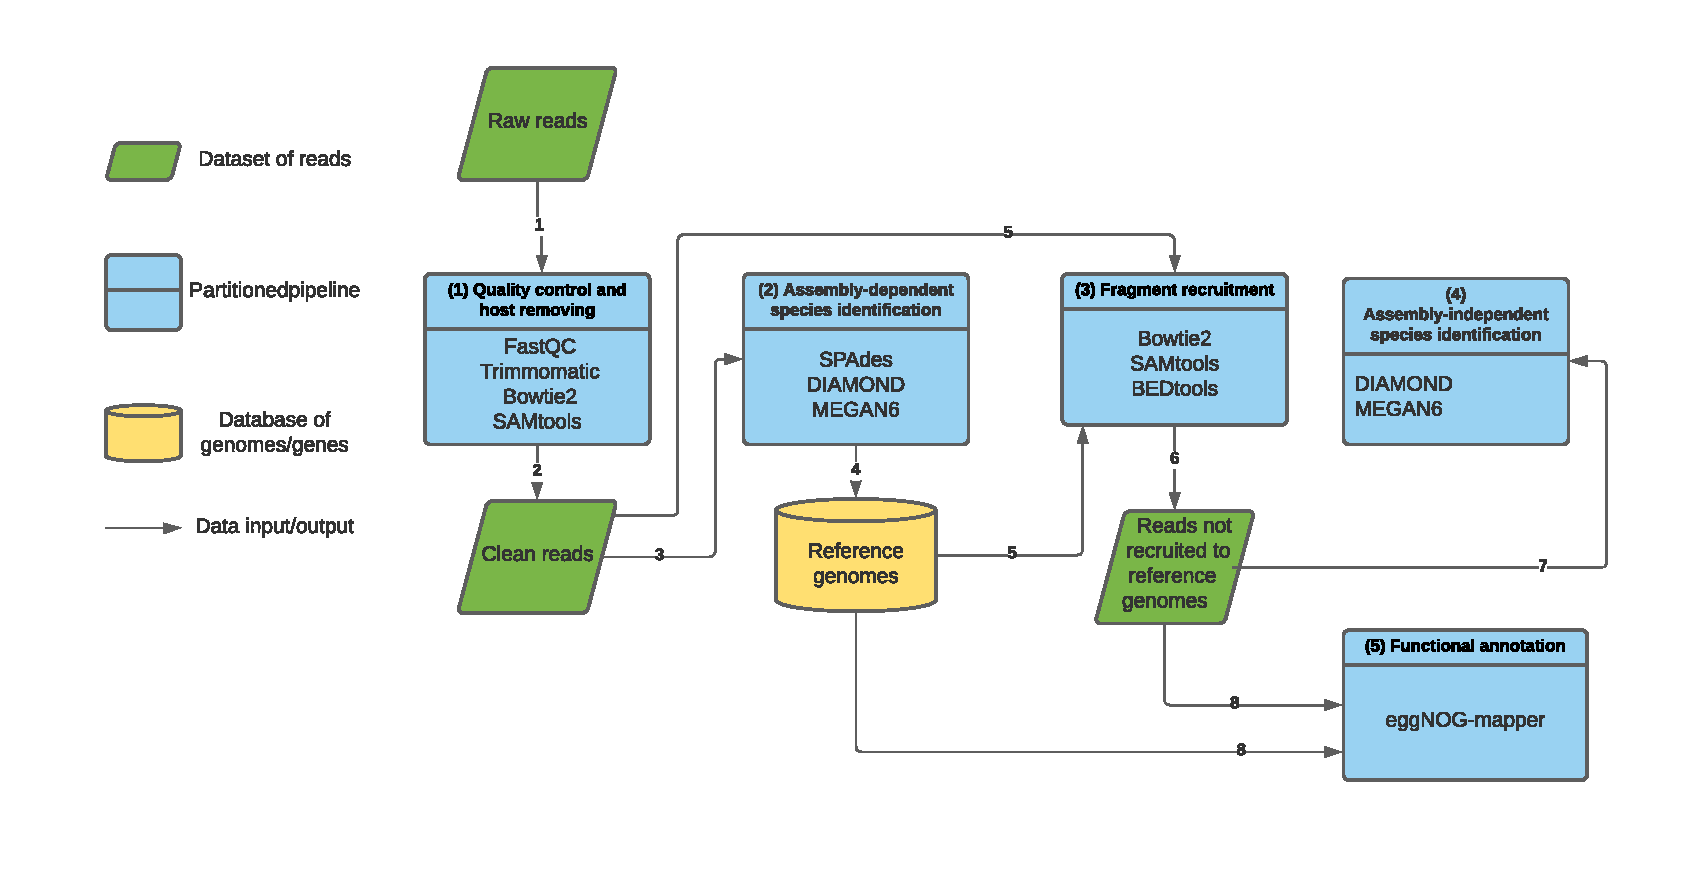
\includegraphics[width=1.1\textwidth]{../Figures/FigurePipeline.pdf}
    \end{figure}
\end{frame}

\begin{frame}{Samples and sequence data}
    \begin{itemize}
        \item Three honey bees (\textit{Apis mellifera})
        \newline Three bumble bees (\textit{Bombus impatiens})
        \newline One flower washes of \textit{Erigeron annuus}
        \item $2 \times 150$bp read pairs
        \item Deep sequencing
        \item Analyzed using the integrated pipeline
    \end{itemize}
%   \begin{table}[htbp!]
%     \centering
%     % \caption{Statistics of sequenced read pairs.}
%     % \label{data_statistics}
%     \resizebox{\textwidth}{!}{
%     \begin{tabular}{@{}ccccc@{}}
%     \hline
%     Sample                           &Host                     &Raw read pair   &\makecell[c]{Clean read pair\\\left[percentage\ of\ raw\ read\ pair\right]}&\makecell[c]{Non-host read pair\\\left[percentage\ of\ clean\ read\ pair]} \\ \hline
%     \textit{Bee\_Amellifera\_hv15\_1}&\textit{Apis mellifera}  &63159968&45059211 \left[71.34\%\right]&38837759 \left[86.19\%\right] \\
%     \textit{Bee\_Amellifera\_wild\_1}&\textit{Apis mellifera}  &58113227&44466776 \left[76.52\%\right]&17014144 \left[38.26\%\right] \\
%     \textit{Bee\_Amellifera\_hv13\_2}&\textit{Apis mellifera}  &56836899&35282101 \left[62.08\%\right]&10413704 \left[29.52\%\right] \\
%     % \textit{Bee\_Amellifera\_hv13\_1}&\textit{Apis mellifera}  &1104861&842095 \left[76.22\%\right]&665507 \left[79.03\%\right] \\
%     \textit{Bee\_Bimpatiens\_hv3\_1} &\textit{Bombus impatiens}&63973750&53612702 \left[83.80\%\right]&5300592 \left[9.89\%\right] \\
%     \textit{Bee\_Bimpatiens\_hv4\_1} &\textit{Bombus impatiens}&58988182&48426748 \left[82.10\%\right]&3557052 \left[7.35\%\right] \\
%     \textit{Bee\_Bimpatiens\_hv4\_2}&\textit{Bombus impatiens} &54955553&45805759 \left[83.35\%\right]&4618023 \left[10.08\%\right] \\
%     \textit{Flower\_eDNA}           &\textit{Erigeron annuus}                      &1443107&882436 \left[61.15\%\right]&882436 \left[100\%\right] \\
%     \hline
%     \end{tabular}
%     }
%     \end{table}
\end{frame}

\begin{frame}{Diverse communities composed of multiple taxonomic clades were identified}
    \begin{figure}[H]
       \includegraphics[width=\textwidth]{../Figures/CommunityClades.png}
        % \caption{The number of host and non-host reads in each sample (a) and the relative abundance of species under six taxonomic groups (b): superkingdom Viruses, superkingdom Bacteria, kingdom Viridiplantae (plants), kingdom Fungi, phylum Arthropoda and others (species that are not in the other five groups).}
        \label{GroupAbundance}
        \end{figure}
\end{frame}

\begin{frame}{Core bacterial symbionts indicates good quality and representativity of samples}
    \begin{figure}[H]
        \centering
        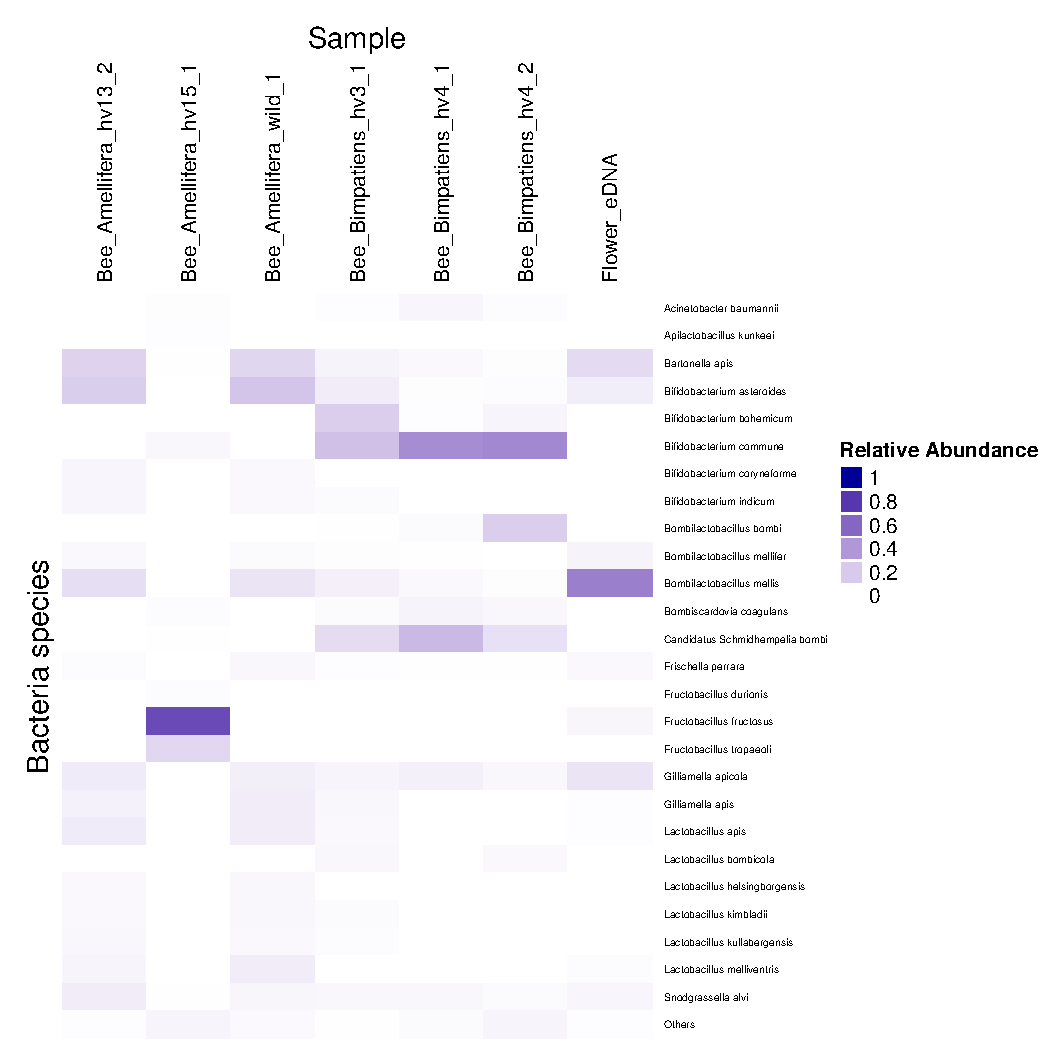
\includegraphics[width=0.7\textwidth]{../Figures/RelativeAbundance_0_01_species_Bacteria.pdf}
        % \caption{Heatmaps for bacterial species abundance distribution in all samples. 
        % The relative abundance takes reads assigned to bacterial species as background. 
        % Species with relative abundance smaller than 1\% in all samples are collapsed as "others".}
        \label{BacteriaHeatmap}
    \end{figure}
\end{frame}

\begin{frame}{Species common in pollination system indicate sample quality and representativity}
    \begin{itemize}
        \item \textcolor{red}{Arthropods}:
        \newline Dominated by \textit{Apis} and \textit{Bombus}
        \item \textcolor{red}{Plants}:
        \newline Crops including rape, soybean, sunflower, radish
        \item \textcolor{red}{Fungi}:
        \newline Dominated by \textit{Nosema ceranae} and yeasts
        \item \textcolor{red}{Viruses}:
        \newline Phages and arthropod-infecting viruses
    \end{itemize}
\end{frame}

% \begin{frame}{Species common in pollination system indicate sample quality and representativity}
%     \begin{figure}
%         \centering
%         \includegraphics[width=0.8\textwidth,height=0.7\textwidth]{../Figures/FungiViruses.png}
%     \end{figure}
% \end{frame}

% \begin{frame}{Species common in pollination system indicate sample quality and representativity}
%     \begin{figure}[H]
%         \centering
%         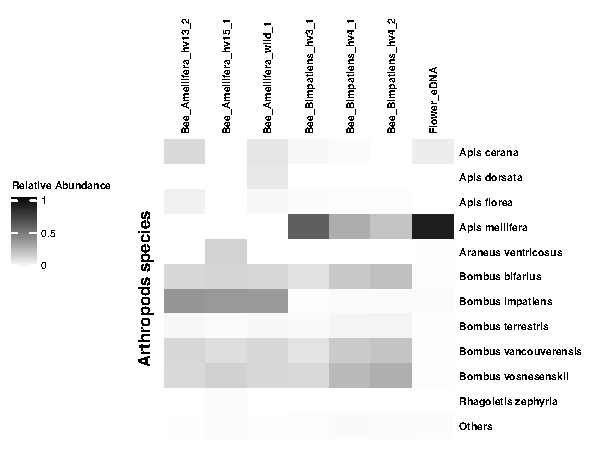
\includegraphics[width=0.7\textwidth]{../Figures/RelativeAbundance_0_01_species_Arthropods.pdf}
%         % \caption{Heatmaps for arthropod species abundance distribution in all samples. 
%         % The relative abundance takes reads assigned to arthropod species as background. 
%         % Species with relative abundance smaller than 1\% in all samples are collapsed as "others". 
%         % It should be noted that for bee samples, host contamination was removed before taxon profiling. 
%         % As a result, the relative abundances of honey bees are extremely low in three honey bee samples, and the same for bumble bees in three bumble bee samples.}
%         % \label{ArthropodHeatmap}
%         \end{figure}
% \end{frame}

% \begin{frame}{Species common in pollination system indicate sample quality and representativity}    
%       \begin{figure}[H]
%         \centering
%         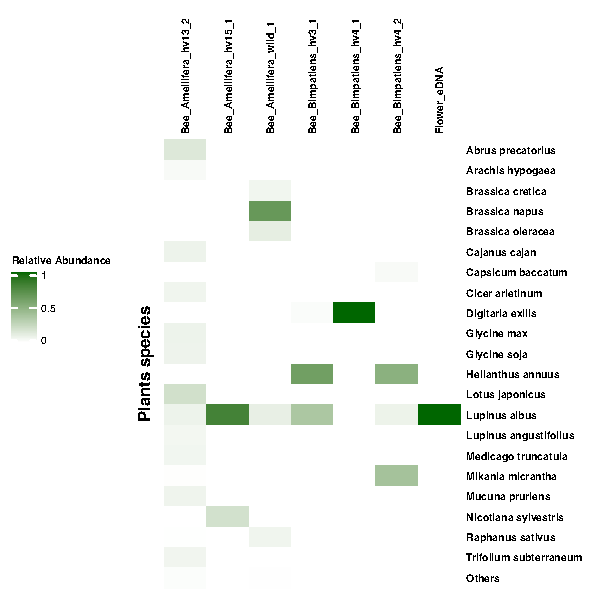
\includegraphics[width=0.7\textwidth]{../Figures/RelativeAbundance_0_01_species_Plants.pdf}
%         % \caption{Heatmaps for plant species abundance distribution in all samples. 
%         % The relative abundance takes reads assigned to plant species as background. 
%         % Species with relative abundance smaller than 1\% in all samples are collapsed as "others".}
%         % \label{PlantHeatmap}
%         \end{figure}
% \end{frame}

% \begin{frame}{Species common in pollination system indicate sample quality and representativity}    
%     \begin{figure}[H]
%       \centering
%       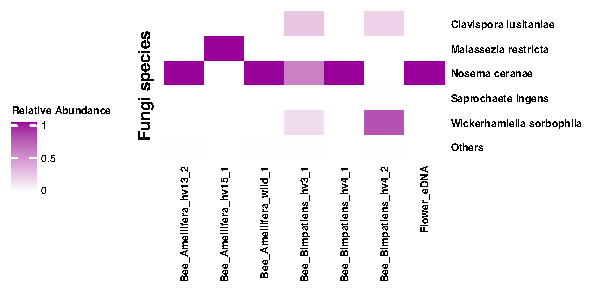
\includegraphics[width=0.7\textwidth]{../Figures/RelativeAbundance_0_01_species_Fungi.pdf}
%       % \caption{Heatmaps for plant species abundance distribution in all samples. 
%       % The relative abundance takes reads assigned to plant species as background. 
%       % Species with relative abundance smaller than 1\% in all samples are collapsed as "others".}
%       % \label{PlantHeatmap}
%       \end{figure}
% \end{frame}

% \begin{frame}{Species common in pollination system indicate sample quality and representativity}    
%     \begin{figure}[H]
%       \centering
%       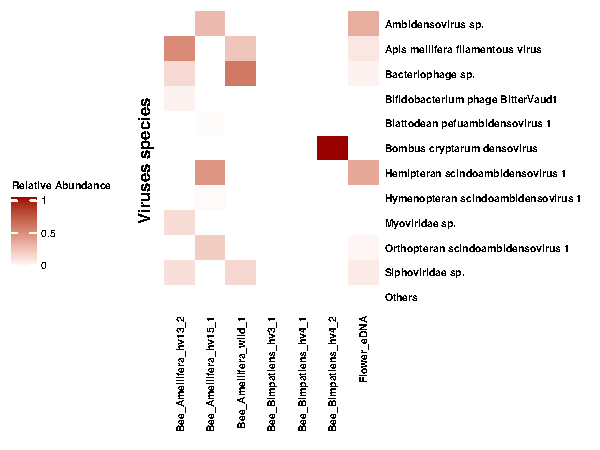
\includegraphics[width=0.7\textwidth]{../Figures/RelativeAbundance_0_01_species_Viruses.pdf}
%       % \caption{Heatmaps for plant species abundance distribution in all samples. 
%       % The relative abundance takes reads assigned to plant species as background. 
%       % Species with relative abundance smaller than 1\% in all samples are collapsed as "others".}
%       % \label{PlantHeatmap}
%       \end{figure}
% \end{frame}

% \begin{frame}{Bee microbime is potentially cabale of metabolizing multiple carbohydrates}
%     \begin{figure}
%         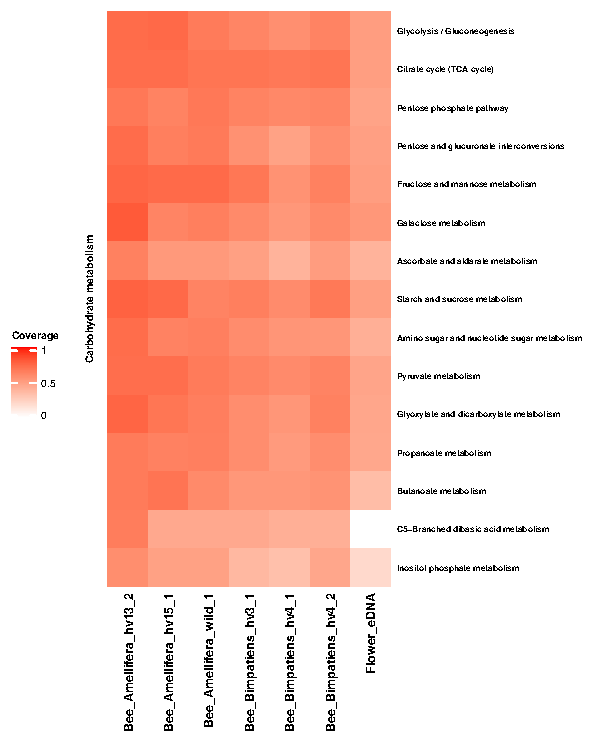
\includegraphics[width=0.6\textwidth]{../Figures/PathwayCov_Carbonhydrate.pdf}
%     \end{figure}
% \end{frame}

% \begin{frame}{Bee microbime is potentially cabale of metabolizing bee essential amino acids}
%     \begin{figure}
%         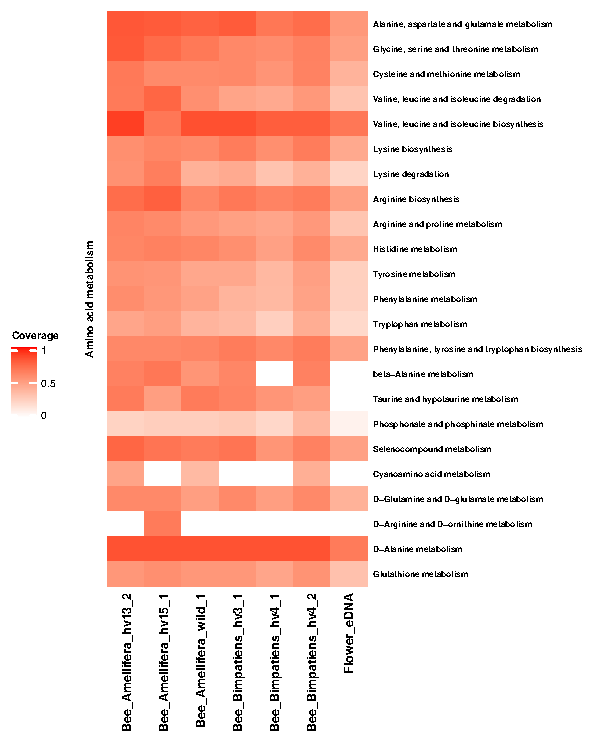
\includegraphics[width=0.6\textwidth]{../Figures/PathwayCov_AminoAcid.pdf}
%     \end{figure}
% \end{frame}

\begin{frame}{Integrated pipeline provided improvement in species identification}
    \begin{figure}
        \includegraphics[width=\textwidth]{../Figures/PipelineEvaluation.png}
        % \caption{Integrated pipeline improves the detection of species richness. 
        % The horizontal axis represents sequencing depth, and the vertical axis represents growth rate of detected species richness comparing the integrated pipeline and assembly-dependent species identification. 
        % Different sequencing depth was simulated by rarefaction.
        % % the ratio between number of novel species detected by assembly-independent search and number of species detected by assembly-dependent search. 
        % Sample type is shown in the top left of each subfigure.}
        % \label{CompareSensitivity}
    \end{figure}
    Sequencing depth was simulated by \newline randomly subsampling original datasets
\end{frame}

\begin{frame}{Advantages of integrated pipeline}
    \begin{itemize}
        \item \textcolor{red}{Improvement in species identification}
        \newline Combination of assembly-free method helps solve species not represented by assembly.
        \item \textcolor{red}{Flexibility}
        \newline Modularity provides capability for incorporating of alternative tools.
        \item \textcolor{red}{Transparency}
        \newline Output files generated by each step are recorded and can be inspected easily for troubleshooting.
    \end{itemize}
\end{frame}

\begin{frame}{Integrated pipeline could be evaluated more comprehensively}
    \begin{itemize}
        \item Microbiome of other host species
        \item Mock metagenomic dataset
        \item Comparison with other strategies, \textit{e.g.} MG-RAST, SqueezeMeta, Kraken. 
    \end{itemize}
\end{frame}

\begin{frame}{Aims}
    \begin{itemize}
        \item Combining assembly-dependent and -independent methods for metagenomic data analysis
        \newline \ \ \ Integrated pipeline
        \item \textcolor{red}{Optimizing sequencing depth to balance sequencing cost and reliable diversity analysis of microbiomes from different host species}
    \end{itemize}
\end{frame}

\begin{frame}{Measure diversity by Hill numbers}
    Hill numbers:
    \begin{equation}
        D^{(q)} = (\sum_{i}^{S}(p_i)^q)^{\frac{1}{1-q}}
        \label{HillNumbers}
      \end{equation}
      $p_i$: the relative abundance of $i$th species or functional gene cluster (KO)
      \newline
      $q$: parameter
      \newline
      $S$: number of categories
      \newline
      \newline
      Advantages:
      \begin{itemize}
          \item Replication principle
          \item Modulate sensitivity to relative abundances via order $q$
          \item Related to widely used diversity indexes:
          \begin{equation}
            D^{(0)} = S
            \end{equation}
            \begin{equation}
                D^{(1)} = e^{-\sum_{i}p_ilogp_i}
            \end{equation}
            \begin{equation}
                D^{(2)} = \frac{1}{\sum_{i}(p_i)^2}
            \end{equation}
      \end{itemize}
\end{frame}

\begin{frame}{Computing expected diversity of given sequencing depth}
    \begin{itemize}
        \item Assume \textcolor{red}{the original datasets is almost complete}
        \newline \textit{i.e.} almost all species/KOs are represented by the original datasets
        \item Simulate shallow sequencing by \textcolor{red}{random subsampling} (10\%-90\% at interval of 10\%)
        \item Fit to \textcolor{red}{asymptotic accumulation models}
        \item \textcolor{red}{Multimodel inference} based on Akaike weight
        \newline 
        \begin{equation}
            D^{(q)}(x) = \sum_{i}w_iD^{(q)}_i(x)
        \end{equation}
        $x$: sequencing depth
        \newline
        $D^{(q)}_i(x)$: $i$th fitted model describing relationship between sequencing depth and Hill numbers
        \newline
        $w_i$: Akaike weight of $i$th model calculated from small sample unbiased Akaike information criterion (AICc)
    \end{itemize}    
\end{frame}

\begin{frame}{Optimizing sequencing depth according to slope of rarefaction curve}
    \begin{figure}
        \includegraphics[width=0.5\textwidth]{../Figures/AccumulationModel.png}
    \end{figure}
    \begin{equation}
        \frac{dD^{q}}{dx} = \sum_{i}w_i\frac{dD^{(q)}_i}{dx}
    \end{equation}
    \begin{equation}
        Asymptote = \lim_{x \to +\infty}D^{(q)}(x)
    \end{equation}
    \begin{equation}
        Completeness = \frac{D^{(q)}(x)}{Asymptote}
    \end{equation}
\end{frame}

\begin{frame}{Verify completeness of original datasets by rarefaction curves for species/KO richness}
    \begin{figure}
        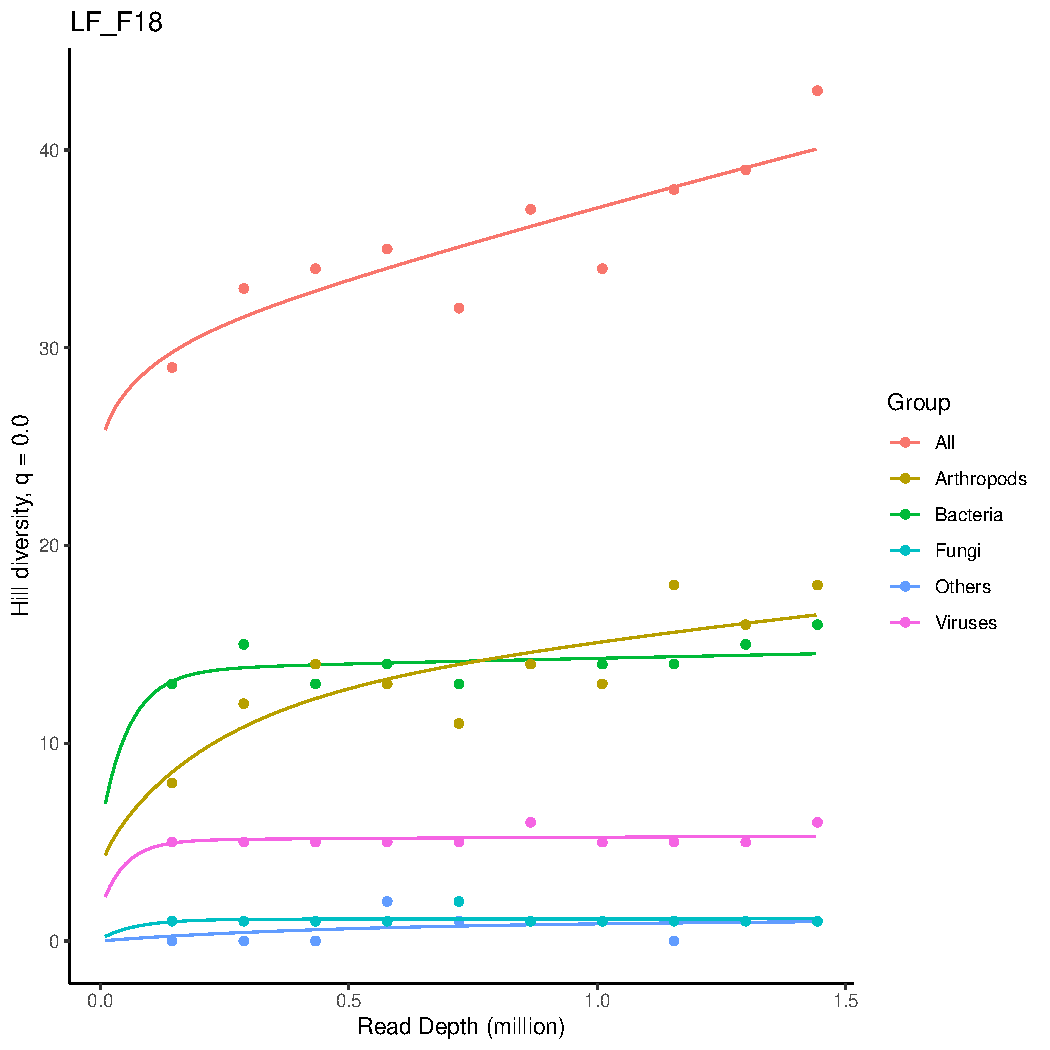
\includegraphics[width=0.9\textwidth]{../Figures/Models.png}
    \end{figure}
\end{frame}

\begin{frame}{Optimal sequencing depth for diversity estimation}
    Species diversity estimation:
    \begin{itemize}
        \item \textit{Bee\_Amellifera\_hv13\_2} and \textit{Flower\_eDNA} were dropped for \textcolor{red}{incompleteness} (final slope $> 1$ and completeness $< 80\%$)
        \item $q = 0$ \textcolor{red}{(species richness)}:
        \newline Slope $< 0.1$ provided completeness $> 95\%$
        \newline Honey bees: 40.33 million (\textcolor{red}{12.10 Gbp})
        \newline Bumble bees: 42.49 million (\textcolor{red}{12.75 Gbp})
        \item $q = 1$ or $2$ \textcolor{red}{(reduced emphasis on rare species)}
        \newline Slope $< 0.01$ provided completeness $> 95\%$
        \newline Honey bees: 18.57 million or \textcolor{red}{5.57 Gbp} ($q = 1$) and 17.45 million or \textcolor{red}{5.24 Gbp} ($q = 2$)
        \newline Bumble bees: 40.33 million or \textcolor{red}{12.10 Gbp} ($q = 1$) and 24.77 million or \textcolor{red}{7.43 Gbp} ($q = 2$)
    \end{itemize}
    Function diversity estimation:
    \begin{itemize}
        \item All datasets were \textcolor{red}{incomplete} (final slope $> 15$)
    \end{itemize}
    
\end{frame}

\begin{frame}{Sequencing depth can be optimized for species diversity estimation}
    Species diversity estimation:
    \begin{itemize}
        \item \textcolor{red}{12.0 Gbp (honey bees)} and \textcolor{red}{12.9 Gbp (bumble bees)} would be sufficient for capturing \textcolor{red}{species richness}
        \item \textcolor{red}{Shallower sequencing} can be adopted when \textcolor{red}{little emphasis} is given on \textcolor{red}{rare species}
    \end{itemize}
    Function diversity estimation:
    \begin{itemize}
        \item \textcolor{red}{Deep sequencing} is valuable
    \end{itemize}
    Limitations:
    \begin{itemize}
        \item Small sample size (3 honey bees, 3 bumble bees and 1 flower eDNA)
        \item Lack of repeat in sequencing depth subsampling
    \end{itemize}
\end{frame}

\begin{frame}{Summary}
    \begin{itemize}
        \item The integrated pipeline provides benefits in terms of \textcolor{red}{results, flexibility and transparency}
        \item For species diversity detection, 12 Gbp for honey bees and 12.9 Gbp for bumble bees would be \textcolor{red}{sufficient}
        \item Shallower sequencing can be adopted with \textcolor{red}{reduced emphasis on rare species}
        \item For function diversity, \textcolor{red}{deep sequencing} would be recommended
        \item Similar \textcolor{red}{pilot studies} for large scale metagenomic project of other host species help budget management
    \end{itemize}
\end{frame}
\end{document}